\begin{frame}
	\frametitle{Markup language e XML}
	\framesubtitle{soluzione corrente per la codifica dei testi}
	\addtocounter{nframe}{1}

	\begin{block}{TEI-XML}
		Le specifiche messe a punto dalla Text Encoding Initiative (TEI-XML) sono considerate ad oggi lo \textbf{standard de facto} per una corretta \textbf{rappresentazione digitale dei testi} con prospettiva accademica.
	\end{block}

\end{frame}

\begin{frame}
	\frametitle{TEI-XML}
	\framesubtitle{Motivazioni per adottare TEI}
	\addtocounter{nframe}{1}

	\begin{block}{Perché TEI}
		La Text Encoding Initiative (\textit{TEI}) è un autorevole \textbf{progetto internazionale}, a cui afferiscono varie \textit{organizzazioni} e \textit{università}, il cui scopo è fornire agli studiosi di informatica umanistica uno strumento il più espressivo e flessibile possibile per rappresentare qualsiasi aspetto di interesse relativo alla \textbf{risorsa testuale da trattare digitalmente}.
	\end{block}

\end{frame}

\begin{frame}
	\frametitle{Introduzione}
	\addtocounter{nframe}{1}
    
    \begin{block}{Qual è l'obiettivo della TEI}
        L'obiettivo della TEI è quello di \textbf{fornire linee guida} per la creazione e la gestione in forma digitale di qualsiasi tipo di dato creato e usato in ambito umanistico.
        \\ E per questo motivo il consorzio investe molte risorse per la accessibilità e la \textbf{divulgazione della tecnologia} che da anni sviluppa.
    \end{block}
    
\end{frame}

\begin{frame}
	\frametitle{I principi fondamentali della TEI}
	\addtocounter{nframe}{1}
    
    \begin{center}
	    
\includegraphics[width=.2\textwidth]{imgs/tei-r.pdf}
	\end{center}

    \begin{itemize}
        
        \item<1-> Le linee guida della TEI privilegiano il ``significato'' (\textbf{meaning}) del testo piuttosto che l'``aspetto'' (layout); privilegia il modello del testo, piuttosto che il formato
          
        \item<2-> La TEI è stata progettata per essere \textbf{indipendente} dagli strumenti software che la usano per la creazione oppure per l'elaborazione dei documenti elettronici

        \item<3-> La TEI cresce, matura, si evolve sulla base delle indicazioni e delle ricerche dalla propria comunità di riferimento (\textbf{community-driven})
           
    \end{itemize}
    
\end{frame}

%%Codifica di testi

% Le norme TEI
% Roberto Rosselli Del Turco
% Dipartimento di Studi Umanistici
% Università di Torino
% roberto.rossellidelturco@fileli.unipi.it
% roberto.rossellidelturco@unito.itLa codifica di testi – Le norme TEI
% La Text Encoding Initiative
% Sito WWW: http://www.tei-c.org/

% \begin{frame}
% 	\frametitle{Intro Text Encoding Initiative}
% 	\framesubtitle{TEI}
% 	\addtocounter{nframe}{1}

% 	\begin{block}{Motto}
% 		TEI: Yesterday's information tomorrow
% 	\end{block}

% 	\begin{block}{Dal sito TEI}
% 		“an international and interdisciplinary standard that
% 		enables libraries, museums, publishers, and individual
% 		scholars to represent a variety of literary and linguistic
% 		texts for online research, teaching, and preservation”
% 	\end{block}
% \end{frame}


\begin{frame}
	\frametitle{Intro Text Encoding Initiative}
	\framesubtitle{TEI}
	\addtocounter{nframe}{1}

	\begin{block}{Testo di riferimento}
        Guidelines for Electronic Text Encoding and Interchange 
        \\( \url{http://www.tei-c.org/Guidelines/} )
	\end{block}

	\begin{block}{testo di ausilio}
		BURNARD, Lou. What is the Text Encoding Initiative? How to add intelligent markup to digital resources. Nouva edizione [online]. Marseille: OpenEdition Press, 2014 (creato il 13 octobre 2018). Disponibile su Internet: \url{http://books.openedition.org/oep/426}. ISBN: 9782821834606. DOI: 10.4000/books.oep.426.

	\end{block}
\end{frame}


% \begin{frame}
% 	\frametitle{Intro Text Encoding Initiative}
% 	\framesubtitle{TEI}
% 	\addtocounter{nframe}{1}

% 	\begin{block}{un po' di storia}
% 		\begin{itemize}
% 			\item 1987: necessità di standard che permetta la creazione e l’interscambio di documenti per mezzo di archivi informatici(convegno NY)
% 			\item 1990: prima versione delle Guidelines (TEI P1)
% 			\item 1990-94: fondi garantiti da enti quali NEH, Mellon Foundation, la Comunità Europea; supporto di ACH, ACL, ALLC
% 		\end{itemize}
% 	\end{block}

% \end{frame}

% \begin{frame}
% 	\frametitle{Intro Text Encoding Initiative}
% 	\framesubtitle{TEI}
% 	\addtocounter{nframe}{1}

% 	\begin{block}{un po' di storia}
% 		\begin{itemize}
% 			\item 2000: nascita del TEI Consortium, associazione non profit per lo sviluppo dello standard TEI
% 			\item 2002: passaggio da SGML a XML con la v. P4
% 			\item 2007: nuova versione TEI P5, continuamente aggiornata
% 		\end{itemize}
% 	\end{block}

% \end{frame}


% \begin{frame}
%     \frametitle{Intro Text Encoding Initiative}
%     \framesubtitle{TEI}
%     \addtocounter{nframe}{1}

% 	\begin{block}{TEI Guidelines}
% 		\textit{versioni P1 e P3 basate su SGML}
% 		\\\textbf{versione P4}
% 		\begin{itemize}
% 			\item standard precedente, ancora impiegata
% 			\item basata su XML, DTD tradizionale
% 			\item pubblicata in forma definitiva nel 2002
% 			\item \url{http://www.tei-c.org/Guidelines/P4/}
% 		\end{itemize}
%     \end{block}
    
% \end{frame}

\begin{frame}
	\frametitle{Intro Text Encoding Initiative}
	\framesubtitle{TEI}
	\addtocounter{nframe}{1}

	\begin{block}{TEI Guidelines: versione P5}
		\begin{itemize}
			\item basata su \textbf{XML}, schema RelaxNG (e DTD tradizionale)
			\item pubblicata alla \textbf{fine del 2007}, aggiornata due volte l’anno
			\item molte novità interessanti (in particolare: maggior \textbf{modularità})
			\item  http://www.tei-c.org/Guidelines/P5/
		\end{itemize}
	\end{block}

\end{frame}

\begin{frame}
	\frametitle{Intro Text Encoding Initiative}
	\framesubtitle{TEI}
	\addtocounter{nframe}{1}

	\begin{block}{TEI Guidelines: Obiettivi}
		\begin{itemize}
			\item better \textbf{interchange} and \textbf{integration} of scholarly data
			\item support for \textit{all texts}, in \textit{all languages}, from \textit{all periods}
			\item guidance for the \textit{perplexed}: \textbf{what to encode} - hence, a user-driven codification of existing best practice
			\item assistance for the \textit{specialist}: \textbf{how to encode} - hence, a loose framework into which unpredictable extensions can be fitted
		\end{itemize}
	\end{block}

\end{frame}



% \begin{frame}
% 	\frametitle{Intro Text Encoding Initiative}
% 	\framesubtitle{TEI}
% 	\addtocounter{nframe}{1}

% 	\begin{block}{TEI Guidelines: Obiettivi}
% 		These apparently incompatible goals result in a highly flexible,
% 		modular, environment for DTD customization.
% 		Lou Burnard, TEI and XML: a marriage made in heaven?
% 		(http://www.tei-c.org/Talks/marriage.xml?style=printable)
% 	\end{block}

% \end{frame}


\begin{frame}
	\frametitle{Intro Text Encoding Initiative}
	\framesubtitle{TEI}
	\addtocounter{nframe}{1}

	\begin{block}{Che cosa offre la TEI}
        \begin{itemize}
            \item un ricco (e complesso) manuale di codifica, 
            \\(le Guidelines for Electronic Text Encoding and Interchange)
            \item un numero elevato di elementi (sia strutturale sia semantico)
            \item schemi di codifica
            \item infrastruttua modulare e personalizzabile
        \end{itemize}

	\end{block}

\end{frame}

% \begin{frame}
% 	\frametitle{Intro Text Encoding Initiative}
% 	\framesubtitle{TEI}
% 	\addtocounter{nframe}{1}

% 	\begin{block}{Che cosa offre la TEI}
% 		\begin{itemize}
% 			\item \textbf{è possibile scegliere soltanto i moduli necessari}
% 			\item \textbf{è possibile modificare le definizioni degli elementi}
% 		\end{itemize}

% 	\end{block}

% \end{frame}

\begin{frame}
	\frametitle{Intro Text Encoding Initiative}
	\framesubtitle{TEI}
	\addtocounter{nframe}{1}

	\begin{block}{Supporto per gli utenti}
		\begin{itemize}
			\item il sito del consorzio (\url{http://www.tei-c.org/})
			\item pagine relative alle varie versioni delle Guidelines
			\item software, tutorial, ecc.
			\item il wiki: \url{http://www.tei-c.org/wiki/index.php/Main_Page}
			\item la mailing list TEI\-L
			\item Github: \url{https://github.com/TEIC}
			\item TEI by example: \url{http://teibyexample.org/}
		\end{itemize}
	\end{block}
\end{frame}


% \begin{frame}
% 	\frametitle{Intro Text Encoding Initiative}
% 	\framesubtitle{TEI}
% 	\addtocounter{nframe}{1}

% 	\begin{block}{Novità della versione P5}
% 		\begin{itemize}
% 			\item modulo di descrizione dei manoscritti
% 			\item grafica e multimedia
% 			\item standoff markup
% 			\item supporto per i namespace XML
% 			\item miglioramenti nel modulo feature structure
% 		\end{itemize}

% 	\end{block}

% \end{frame}

% \begin{frame}
% 	\frametitle{Intro Text Encoding Initiative}
% 	\framesubtitle{TEI}
% 	\addtocounter{nframe}{1}

% 	\begin{block}{Novità della versione P5 (cont.)}
% 		\begin{itemize}
% 			\item modulo di descrizione dei manoscritti
% 			\item grafica e multimedia
% 			\item standoff markup
% 			\item supporto per i namespace XML
% 			\item miglioramenti nel modulo feature structure
% 		\end{itemize}

% 	\end{block}

% \end{frame}

\begin{frame}
	\frametitle{Intro Text Encoding Initiative}
	\framesubtitle{TEI}
	\addtocounter{nframe}{1}

	\begin{block}{TEI: Struttura modulare}
		\begin{itemize}
			\item si scelgono soltanto i \textbf{moduli che corrispondono alle proprie esigenze}, in modo da realizzare rapidamente uno schema di codifica appropriato
			\item ogni modulo contiene un certo numero di \textbf{elementi} (\textit{tagset})
			\item gli \textbf{elementi} sono organizzati in \textbf{classi} (strutturali, semantiche)
			\item gli \textbf{attributi} sono organizzati in \textbf{classi} (globali e specifici)
		\end{itemize}

	\end{block}

\end{frame}


% classi strutturali: elementi che hanno un ruolo a livello strutturale
% (paragrafi, strofe, etc.)
% classi semantiche: elementi descrittivi del testo (aggiunte,
% correzioni, nomi di persona, etc.)
% anche gli attributi sono organizzati in classi
% attributi globali: disponibili per tutti gli elementi
% attributi specifici: solo per alcuni elementi


\begin{frame}
	\frametitle{Intro Text Encoding Initiative}
	\framesubtitle{TEI}
	\addtocounter{nframe}{1}

	\begin{block}{TEI: Struttura modulare - Moduli essenziali}
		\begin{itemize}
			\item \textbf{tei}: definisce le classi di elementi, le macro e i datatype che verranno usati per tutti i moduli
			\item \textbf{header}: l’intestazione contenente i metadati relativi al documento TEI XML
			\item \textbf{textstructure}: elementi strutturali per qualsiasi tipo di testo
			\item \textbf{core}: elementi utili in qualsiasi tipo di documento
		\end{itemize}

	\end{block}

\end{frame}

\begin{frame}
	\frametitle{Intro Text Encoding Initiative}
	\framesubtitle{TEI}
	\addtocounter{nframe}{1}

	\begin{block}{TEI: Struttura modulare - Moduli facoltativi}
		\begin{itemize}
			\item \textbf{analysis}: strumenti per analisi (linguistica etc.) del testo
			\item \textbf{corpus}: gestione di corpora linguistici
			\item \textbf{drama}: elementi per testi teatrali e drammatici
			\item \textbf{gaiji}: rappresentazione di caratteri e glifi non standard
			\item \textbf{msdescription}: metadati relativi a manoscritti
		\end{itemize}

	\end{block}

\end{frame}


\begin{frame}
	\frametitle{Intro Text Encoding Initiative}
	\framesubtitle{TEI}
	\addtocounter{nframe}{1}

	\begin{block}{TEI: Struttura modulare - Moduli facoltativi}
		\begin{itemize}
			\item \textbf{spoken}: trascrizione del parlato
			\item \textbf{textcrit}: apparato critico
			\item \textbf{transcr}:  trascrizione di fonti primarie (manoscritti)
			\item \textbf{verse}: elementi supplementari per testi poetici
		\end{itemize}

	\end{block}

\end{frame}

% \begin{frame}
% 	\frametitle{Intro Text Encoding Initiative}
% 	\framesubtitle{TEI}
% 	\addtocounter{nframe}{1}

% 	\begin{block}{TEI Lite}

% 		una specifica \textbf{personalizzazione} della TEI versione P4/5

% 	\end{block}

% 	\textit{A simple demonstration of how the TEI encoding scheme
% 		might be adopted to meet 90\% of the needs of 90\% of the
% 		TEI user community (dalla Prefatory Note: \\url{http://www.tei-
% 		c.org/Lite/})}

% \end{frame}


% \begin{frame}
% 	\frametitle{Intro Text Encoding Initiative}
% 	\framesubtitle{TEI}
% 	\addtocounter{nframe}{1}

% 	\begin{block}{TEI Lite}

% 		La \textbf{versione P4} è stata tradotta anche in italiano: TEI Lite:
% 		introduzione alla codifica dei testi, a cura di \textit{F. Ciotti} (
% 		\url{http://www.tei-c.org/Lite/teiu5_it.html}).
%     \end{block}
%     \textit{Molto usata, ma presenta varie limitazioni, con la versione P5 è più semplice produrre una versione semplificata o personalizzata}
% \end{frame}

% \begin{frame}
% 	\frametitle{Intro Text Encoding Initiative}
% 	\framesubtitle{TEI}
% 	\addtocounter{nframe}{1}

% 	\begin{block}{TEI Pizza chef}

% 		la TEI P4 poteva essere modificata usando un programma su
% 		web chiamato Pizza chef
% 		\url{http://www.tei-c.org.uk/pizza.html}.
% 		\\Metafora della base e dei condimenti (toppings),
% 		corrispondenti ai moduli indispensabili e a quelli facoltativi.
% 		\\Meccanismo efficace, soprattutto considerando l’alternativa
% 		(modifica manuale delle DTD TEI).
%     \end{block}
    
%     \textit{Tool obsoleto, necessaria comunque modifica manuale per nuovi elementi}


% \end{frame}

% \begin{frame}
% 	\frametitle{Intro Text Encoding Initiative}
% 	\framesubtitle{TEI}
% 	\addtocounter{nframe}{1}

% 	\begin{block}{TEI Roma}

% 		Per la P5 si è deciso di proporre una modularizzazione più
% 		efficace, e uno strumento di personalizzazione più potente.
% 		Strumento basato sul nuovo formato ODD.


% 	\end{block}

% 	\begin{block}{TEI Roma}
% 		Il metodo da seguire per la versione P5 (quella che
% 		useremo) fino all’arrivo del successore (Byzantium)

% 	\end{block}

% \end{frame}

% \begin{frame}
% 	\frametitle{Intro Text Encoding Initiative}
% 	\framesubtitle{TEI}
% 	\addtocounter{nframe}{1}

% 	\begin{block}{TEI Roma}

% 		\begin{itemize}
% 			\item  possibilità di scegliere, escludere, modificare sia gli elementi (e le classi di elementi), sia gli attributi (e le classi di attributi)
% 			\item possibilità di aggiungere elementi (eventualmente inserendoli nelle classi preesistenti)
% 			\item possibilità di salvare lo schema in tre formati diversi: DTD  tradizionale, W3C e RelaxNG (anche in forma compatta)
% 		\end{itemize}

% 	\end{block}


% \end{frame}


% \begin{frame}
% 	\frametitle{Intro Text Encoding Initiative}
% 	\framesubtitle{TEI}
% 	\addtocounter{nframe}{1}

% 	\begin{block}{TEI Roma: Il formato ODD}
% 		le versioni P1 – P4 delle DTD TEI erano nel formato DTD language e dipendevano dalla sintassi SGML per molti aspetti
% 	\end{block}

% 	\begin{block}{TEI Roma: Il formato ODD}
% 		One Document Does it all (ODD): set di specifiche in base alle quali un semplice documento TEI XML \textit{“defines a schema in terms of the modules it requires, together with any possible modifications, such as the desired
%         root element”}. 
%     \end{block}
    
%     \textbf{Risultato finale: lo schema nel linguaggio desiderato e la relativa documentazione}

% \end{frame}


\begin{frame}
	\frametitle{Intro Text Encoding Initiative}
	\framesubtitle{TEI}
	\addtocounter{nframe}{1}

	\begin{block}{TEI Roma: Il formato ODD}

		tutorial: Getting Started with P5 ODDs\\
		\url{http://www.tei-c.org/Guidelines/Customization/odds.xml}

	\end{block}


\end{frame}


% 15La codifica di testi – Le norme TEI
% TEI Roma 2
% per motivi vari, la manutenzione di TEI Roma lascia a
% desiderare (per non parlare dello sviluppo di un successore)
% nel passato recente la componente di “controllo” dello
% schema (Sanity checker) non funzionava
% in tal caso è possibile andare sul sito TEI di Oxford dove è in
% esecuzione una versione più vecchia:
% http://tei.it.ox.ac.uk/Roma/
% Roma, in ogni caso, è solo un front-end per il linguaggio ODD
% (cfr. infra)




\begin{frame}
	\frametitle{Intro Text Encoding Initiative}
	\framesubtitle{TEI}
	\addtocounter{nframe}{1}

	\begin{block}{Il futuro della TEI}
		\textbf{negli ultimi anni gli schemi TEI sono stati oggetto di alcune critiche}
	\end{block}

	\begin{block}{Il futuro della TEI}
		\begin{itemize}
			\item la TEI è troppo grande / complicata / piccola
			\item la TEI è basata su XML e questo formato è in declino
			\item la TEI/XML non supporta le gerarchie multiple
			\item la TEI non supporta il markup di tipo stand-off
		\end{itemize}
	\end{block}

\end{frame}


\begin{frame}
	\frametitle{Intro Text Encoding Initiative}
	\framesubtitle{TEI}
	\addtocounter{nframe}{1}

	\begin{block}{Il futuro della TEI}
		la cosa importante da ricordare è che se c’è una discrepanza fra Guidelines TEI e schemi di codifica, la precedenza va alle Guidelines (livello di astrazione del modello TEI)
	\end{block}

\end{frame}


\begin{frame}
	\frametitle{Intro Text Encoding Initiative}
	\framesubtitle{TEI}
	\addtocounter{nframe}{1}

	\begin{block}{text encoding con la TEI}
		E' caldamente raccomandato usare direttamente la
		versione più recente della P5.\\
		La flessibilità della P5 permette di definire uno schema di
		codifica che corrisponda precisamente al modello
    \end{block}
    
    \textit{La comunità di utenti e sviluppatori TEI offre un buon supporto.}

\end{frame}


%%%%%%%%%%%%%%%%%%%%%%
% Codifica di testi
% I moduli base della TEI
% Roberto Rosselli Del Turco
% Dipartimento di Studi Umanistici
% Università di Torino
% roberto.rossellidelturco@fileli.unipi.it
% roberto.rossellidelturco@unito.itSchemi di codifica TEI – Moduli base
% Elementi disponibili per tutti i documenti TEI

\begin{frame}
	\frametitle{Intro Text Encoding Initiative}
	\framesubtitle{TEI}
	\addtocounter{nframe}{1}

	\begin{block}{Un documento TEI P5 ‘minimo’}
        \begin{itemize}
            \item prologo XML
            \item intestazione TEI
            \item elementi strutturali
            \item elementi semantici dei moduli base
        \end{itemize}
    \end{block}
    
\end{frame}

\begin{frame}
	\frametitle{Intro Text Encoding Initiative}
	\framesubtitle{TEI}
	\addtocounter{nframe}{1}

   \textbf{ Moduli di base: \textit{tei}, \textit{header}, \textit{textstructure}, \textit{core}}

	\begin{block}{un documento TEI P5 ‘minimo’}
        Anche usando soltanto i moduli essenziali si ha a disposizione
        uno schema adatto alla marcatura di numerosi tipi di testi.
    \end{block}
 
       \textit{Schemi ``leggeri'' consigliati: la TEI Lite, o se necessario una
        versione più ridotta della P5 (TEI
        Absolutely Bare)}
\end{frame}





\begin{frame}
    \frametitle{Infrastruttura TEI}
    \framesubtitle{Tabella Moduli TEI}
    \addtocounter{nframe}{1}
    
    \begin{block}{TEI framework}
        
            La tecnologia TEI ha un framework concettuale diviso in
                \begin{itemize}
                    \item Moduli
                    \item Classi
                    \item Macro
                    \item Tipi di Dato
                \end{itemize}

    \end{block}
\end{frame}


\begin{frame}
    \frametitle{Infrastruttura TEI}
    \framesubtitle{Tabella Moduli TEI}
    \addtocounter{nframe}{1}
    
    \begin{block}{Moduli TEI}
        Un modulo è semplicemente un contenitore per una serie di dichiarazioni uniformi e coerenti per gli elementi TEI e le relative classi.
    \end{block}
\end{frame}

\begin{frame}
    \frametitle{Infrastruttura TEI}
    \framesubtitle{Tabella Moduli TEI}
    \addtocounter{nframe}{1}
    
        \begin{center}
        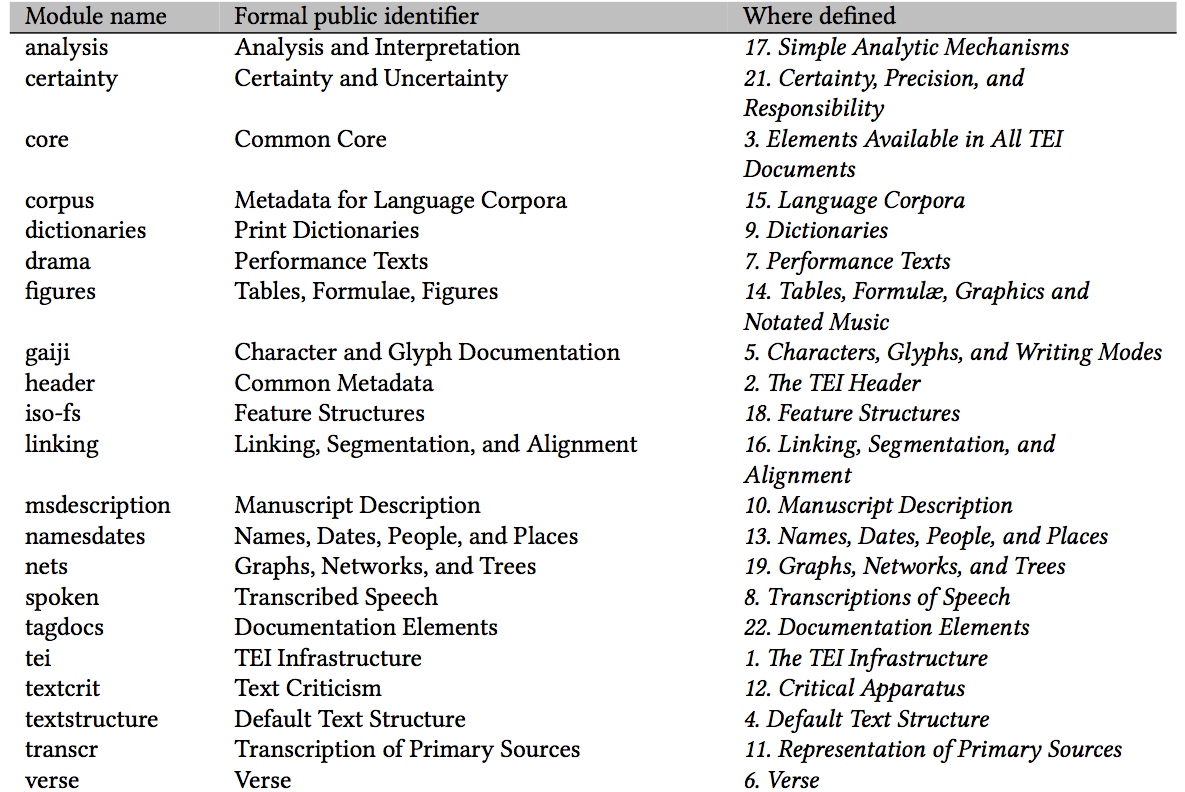
\includegraphics[width=.95\textwidth]{imgs/ModuliTEI.png}
        \end{center}
   
\end{frame}

\begin{frame}
    \frametitle{Infrastruttura TEI}
    \framesubtitle{Tabella Moduli TEI}
    \addtocounter{nframe}{1}
        \begin{center}
        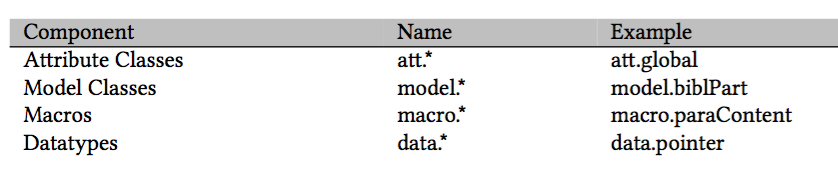
\includegraphics[width=.95\textwidth]{imgs/ModelloTEI.png}
        \end{center}
\end{frame}

\begin{frame}
    \frametitle{Infrastruttura TEI}
    \framesubtitle{Tabella Moduli TEI}
    \addtocounter{nframe}{1}
    
    \begin{block}{Classi TEI}
        Le classi sono usate per esprimere due distinti tipi di \textbf{caratteristiche comuni} ad un insieme di elementi. 
    \end{block}

    \begin{block}{Classi TEI}
        Gli elementi di una classe possono \textit{condividere un insieme di attributi} oppure possono far \textit{parte di uno stesso content model}.
    \end{block}
\end{frame}

\begin{frame}
    \frametitle{Infrastruttura TEI}
    \framesubtitle{Tabella Moduli TEI}
    \addtocounter{nframe}{1}
    
    \begin{block}{Classi TEI}
        \begin{itemize}
            \item Un elemento appartenente ad una classe attributo condivide gli attributi con tutti gli altri elementi membri della stessa classe. 
            \item Un elemento appartenente alla classe modello condivide il luogo del content model dove appare con gli altri elementi membri della stessa classe.
        \end{itemize}
    \end{block}
    \textit{ In entrambi i casi un \textbf{elemento eredita} proprietà dalle classi di cui è membro.}
\end{frame}

\begin{frame}
    \frametitle{Infrastruttura TEI}
    \framesubtitle{Tabella Moduli TEI}
    \addtocounter{nframe}{1}
        \begin{center}
        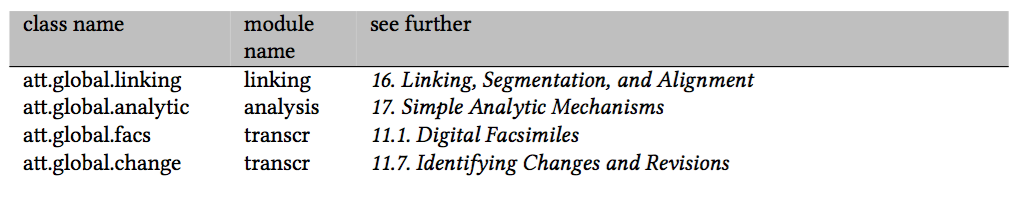
\includegraphics[width=.95\textwidth]{imgs/Classi-AttributiGlobaliModuli.png}
        \end{center}
\end{frame}


\begin{frame}
    \frametitle{Infrastruttura TEI}
    \framesubtitle{Tabella Moduli TEI}
    \addtocounter{nframe}{1}
    
    \begin{block}{Macro TEI}
        Le Macro sono shortcut per dichiarazioni che occorrono frequentemente. 
        \\ Le Macro sono utilizzate in due modi diversi:
        \begin{itemize}
            \item per content model o parti di content model \textit{frequently-encountered}
            \item per datatype di attributi
        \end{itemize}
         
    \end{block}
\end{frame}

\begin{frame}
    \frametitle{Infrastruttura TEI}
    \framesubtitle{Tabella Moduli TEI}
    \addtocounter{nframe}{1}
    
    \begin{block}{Data Type TEI}
        I valori che possono assumere gli attributi sono definiti da tipi di dato all'interno delle \textit{TEI datatype specification}.
    \end{block}

    \begin{block}{Data Type TEI}
       
    \end{block}
    Le specifiche TEI definiscono i propri tipi di dato sfruttando altri tipi di dato primitivi e quelli derivati dalle specifiche W3C. 
\end{frame}





% xx sezione 1 frame 01
% \begin{frame}
%     \frametitle{Attributi Globali}
%     \framesubtitle{Elenco}
%     \addtocounter{nframe}{1}


% \textbf{\textrm{att.global} provides attributes common to all elements in the TEI encoding scheme.}

% \begin{description}
%     \item [@xml:id]     \textbf{identifier} provides a unique identifier for the element bearing the attribute.
%     \item [@n]          \textbf{number} gives a number (or other label) for an element, which is not necessarily unique within the document.
%     \item [@xml:lang]   \textbf{language} indicates the language of the element content using a ‘tag’ generated according to BCP 47\footnote{see \href{http://google.con}{http://google.com}}.
% \end{description}

% \end{frame}


% % xx sezione 1 frame 02
% \begin{frame}
%     \frametitle{Attributi Globali}
%     \framesubtitle{Elenco cont..}
%     \addtocounter{nframe}{1}


% \textbf{\textmd{att.global} provides attributes common to all elements in the TEI encoding scheme.}

% \begin{description}
%     \item [rend] [att.global.rendition]	(rendition) indicates how the element in question was rendered or presented in the source text.
%     \item [style] [att.global.rendition]	contains an expression in some formal style definition language which defines the rendering or presentation used for this element in the source text
%     \item [rendition] [att.global.rendition]	points to a description of the rendering or presentation used for this element in the source text.
% \end{description}

% \end{frame}

% % xx sezione 1 frame 03
% \begin{frame}
%     \frametitle{Attributi Globali}
%     \framesubtitle{Elenco cont...}
%     \addtocounter{nframe}{1}


% \textbf{\textmd{att.global} provides attributes common to all elements in the TEI encoding scheme.}

% \begin{description}
%     \item [xml:base]	provides a base URI reference with which applications can resolve relative URI references into absolute URI references.
%     \item [xml:space]	signals an intention about how white space should be managed by applications.
%     \item [source] [att.global.source]	specifies the source from which some aspect of this element is drawn.
% \end{description}

% \end{frame}

% % xx sezione 1 frame 04
% \begin{frame}
%     \frametitle{Attributi Globali}
%     \framesubtitle{Elenco cont....}
%     \addtocounter{nframe}{1}


% \textbf{\textmd{att.global} provides attributes common to all elements in the TEI encoding scheme.}

% \begin{description}
%     \item [cert] [att.global.responsibility]	(certainty) signifies the degree of certainty associated with the intervention or interpretation.
%     \item [resp] [att.global.responsibility]	(responsible party) indicates the agency responsible for the intervention or interpretation, for example an editor or transcriber.
% \end{description}

% \end{frame}


% xx sezione 1 frame 05

% \begin{frame} [fragile]
%     \frametitle{Attributi Globali}
%     \framesubtitle{Esempio \textrm{@xml:lang}}
%     \addtocounter{nframe}{1}

%     \textbf{\textrm{xml:lang} indica la lingua e il sistema di scrittura usato}
%     \defverbatim{\langatt}{%
%         \begin{tiny}
%         \begin{verbatim}
%             <TEI xmlns="http://www.tei-c.org/ns/1.0">
%                 <teiHeader xml:lang="en">
%                     <!-- ... -->
%                 </teiHeader>
%                 <text xml:lang="fr">
%                     <body>
%                         <div>
%                             <!-- chapter one is in French -->
%                         </div>
%                         <div xml:lang="de">
%                             <!-- chapter two is in German -->
%                         </div>
%                         <div>
%                             <!-- chapter three is French -->
%                         </div>
%                         <!-- ... -->
%                     </body>
%                 </text>
%             </TEI>
%         \end{verbatim}
%         \end{tiny}
%         }
%         \begin{center}
%             {\langatt}
%         \end{center}
% \end{frame}


% % xx sezione 1 frame 06
% \begin{frame}
%     \frametitle{Attributi Globali}
%     \framesubtitle{Stile e Aspetto}
%     \addtocounter{nframe}{1}

    
%     \textbf{In the TEI scheme, it is possible to supply information about the appearance of elements within a source document in the following distinct ways:}

%     \begin{itemize}
%         \item One or more properties may be specified as the default for a set of elements (based on an external scheme, by default CSS), using rendition elements and their selector attributes;
%         \item One or more properties may be specified for individual element occurrences, using the rend attribute with any convenient set of one or more sequence-indeterminate tokens;
%     \end{itemize}
% \end{frame}

% % xx sezione 1 frame 07
% \begin{frame}
%     \frametitle{Attributi Globali}
%     \framesubtitle{Stile e Aspetto cont..}
%     \addtocounter{nframe}{1}
    
%     \textbf{Note that these TEI attributes always describe the rendition or appearance of the source document, not intended output renditions, although often the two may be closely related.}

%     \begin{itemize}
%         \item One or more properties may be specified for individual element occurrences, using the rendition attribute to point to rendition elements;
%         \item One or more properties may be supplied explicitly for individual element occurrences, using the style attribute.
%     \end{itemize}

% \end{frame}


% xx sezione 1 frame 08

% \begin{frame}
%     \frametitle{Attributi Globali}
%     \framesubtitle{da vari altri Moduli Tabella}
%     \addtocounter{nframe}{1}
%     %fare una tabella 
% class name	module name	see further
% att.global.linking	linking	16 Linking, Segmentation, and Alignment
% att.global.analytic	analysis	17 Simple Analytic Mechanisms
% att.global.facs	transcr	11.1 Digital Facsimiles
% att.global.change	transcr	11.7 Identifying Changes and Revisions

% \end{frame}

%%%%%%%%%%
% attributi globali: source, cert, resp, xml:base, xml:space
% Altri attributi Globali divisi per classe e per moduli.
% Appendice A per lista alfabetica delle Classi di Modello.

%% Macro e DataType
% Tabella Macro
% 


\begin{frame}
    \frametitle{Infrastruttura TEI}
    \framesubtitle{Classificazione degli elementi}
    \addtocounter{nframe}{1}
    \textit{Quasi tutti gli elementi TEI possono essere \textbf{classificati informalmente} come appartenenti alle seguenti categorie:}
    \begin{block}{TEI element classification}
        \begin{itemize}
            \item divisions
            \item chunks
            \item phrase-level elements
            \item inter-level elements
            \item components
        \end{itemize}

    \end{block}

\end{frame}

\begin{frame}
    \frametitle{Infrastruttura TEI}
    \framesubtitle{Classificazione degli elementi}
    \addtocounter{nframe}{1}
   
    \begin{itemize}
       \item \textbf{divisions}
       \item[] Divisioni ad alto livello dei testi, molto spesso elementi annidati.
    \end{itemize}

   \begin{itemize}
    \item \textbf{chunks}
    \item[] Elementi come i paragrafi e altri elementi simili i quali sono posizionati all'interno dei testi e divisioni. Solitamente non sono elementi che possono annidarsi o apparire all'interno di altri elementi di livello chunk.
    \end{itemize}

\end{frame}


\begin{frame}
    \frametitle{Infrastruttura TEI}
    \framesubtitle{Classificazione degli elementi}
    \addtocounter{nframe}{1}
   

    \begin{itemize}
        \item \textbf{phrase-level elements}
        \item[] Elementi che occorrono solo all'interno di elementi di livello chunk.
     \end{itemize}
 
    \begin{itemize}
     \item \textbf{inter-level elements}
     \item[] Elementi che possono occorrere sia tra chunks all'interno di division, sia all'interno di essi.
     \end{itemize}

     \begin{itemize}
        \item \textbf{components}
        \item[] Elementi che possono occorrere direttamente all'interno dei testi o delle divisioni di testo. E' una combinazione di elementi di livello inter e chunk.
        \end{itemize}
   
\end{frame}


\begin{frame}
	\frametitle{Intro Text Encoding Initiative}
	\framesubtitle{Schemi di codifica TEI – Moduli base}
	\addtocounter{nframe}{1}

	\begin{block}{Struttura di un documento TEI}
        \begin{itemize}
            \item \textit{struttura fondamentale all’interno della radice (\texttt{<TEI>})}
            \item una intestazione TEI (\texttt{<teiHeader>})
            \item un testo: \texttt{<text>} (o più testi, cfr. infra)
        \end{itemize}
    \end{block}
    
\end{frame}




%%%%% PORTARE DOPO XML %%%%%%%
%%                          %%



 
